% ============================================================
% File:    job_talk.tex
% Purpose: 30-slide beamer job-talk version of main.tex
% Inputs:  ../../output/reg/*_present.tex, ../../output/sum/*_present.tex,
%          ../../output/fig/*.png, img/*, citation.bib
% Outputs: job_talk.pdf
% Author:  EK  Date: 2026-08-31
% ============================================================

\documentclass{beamer}
\usetheme{Boadilla}
\setbeamertemplate{footline}[page number]
\setbeamertemplate{navigation symbols}{}

\usepackage{graphicx}
\usepackage{booktabs}
\usepackage{array}
\usepackage{adjustbox}
\usepackage{varwidth}
\usepackage{amsmath}
\usepackage{amssymb}

\usepackage[
backend=biber,
style=authoryear,
citestyle=bwl-FU
]{biblatex}
\addbibresource{citation.bib}

% ============================================================
% Pipeline output directory (relative to this file)
%   \presreg{name}  -> ../../output/reg/name_present.tex
%   \pressum{name}  -> ../../output/sum/name_present.tex
%   \presfig{f.png} -> ../../output/fig/f.png
% ============================================================
\newcommand{\outputdir}{../../output}

% The generated *_present.tex files are written as article floats:
% \begin{table}[htbp] ... \caption{...} ... \end{table}. Beamer has no float
% mechanism, and wrapping a float in adjustbox raises
% "! LaTeX Error: Not in outer par mode." Neutralise the float and swallow the
% caption (on a slide the frame title carries the caption text), so the table
% body is plain material that can be boxed and scaled.
\makeatletter
\renewenvironment{table}[1][]{\par\centering}{\par}
\renewcommand{\caption}[2][]{}
\makeatother

% Box the table body at its natural width inside a varwidth, so multi-panel
% files still break between panels instead of setting them side by side, then
% shrink only as much as is needed to fit the slide.
% Optional argument overrides the width key, for source files that hardcode a
% narrow adjustbox (e.g. width = 0.45\textwidth) and so need scaling UP: max
% width only ever shrinks.
\newcommand{\slidetableinput}[2][max width=\textwidth]{%
  \adjustbox{#1, max totalheight=0.80\textheight, center}{%
    \begin{varwidth}{17cm}%
      \input{#2}%
    \end{varwidth}}}
\newcommand{\presreg}[2][max width=\textwidth]{\slidetableinput[#1]{\outputdir/reg/#2_present}}
\newcommand{\pressum}[2][max width=\textwidth]{\slidetableinput[#1]{\outputdir/sum/#2_present}}
\newcommand{\presfig}[2][0.75\textheight]{%
  \begin{center}%
  \adjustbox{max width=\textwidth, max height=#1}{\includegraphics{\outputdir/fig/#2}}%
  \end{center}}

% One-line takeaway under a table or figure. The group must close AFTER \par or
% the paragraph inherits the outer font's baselineskip on its first line.
\newcommand{\takeaway}[1]{\par\medskip{\footnotesize #1\par}}

\AtBeginSection[]{
  \begin{frame}
  \vfill
  \centering
  \begin{beamercolorbox}[sep=8pt,center,shadow=true,rounded=true]{title}
    \usebeamerfont{title}\insertsectionhead\par%
  \end{beamercolorbox}
  \vfill
  \end{frame}
}

\title[Contamination and Self-Reported Compliance]{The Effect of Contamination on Contamination Limit Regulation}
\subtitle{US Coal Mining and Drinking Water Utilities}
\author{Emil Kee-Tui}
\institute{Charles H. Dyson School of Applied Economics and Management \\ Cornell University}
\date{September 2026}

\begin{document}

% ---------------------------------------------------------------- 1
\begin{frame}
\titlepage
\end{frame}

\begin{frame}{US drinking water is monitored through self-reports}
\begin{itemize}
    \item Drinking water utilities provide treated water from groundwater and/or surface water sources to twenty five to millions of customers, publicly or privately owned.
    \item 85\% of US households obtain water from a utility required to treat and self-report water quality.
    \begin{itemize}
        \item Testing requires technical staff, administrative tracking, and laboratories.
        \item Self-reporting is a larger burden than the MCL (\cite{oleckno1982national}).
        \item Testing \textbf{requirements increase with assessed source-water impairment}.
    \end{itemize}
    \item 9 to 34 million US households obtain water from a utility violating a health standard \parencite{allaire2018national}.
\end{itemize}
\end{frame}

\begin{frame}{Self-reported compliance}
\begin{itemize}
    \item Personal income taxes, Healthcare HIPAA violation disclosure, energy firms self-report anti-competitiveness/negligence to the Federal Energy Regulatory Commission, public companies' Sarbanes‑Oxley Act self-report financial statement accuracy, Toxic Release Inventories, and drinking water utilities.
    \item The regulator learns of a violation if the firm self-reports.
    \item Water quality violations:
    \begin{itemize}
        \item \textbf{MCL} --- reported contamination above the limit. Formally enforced.
        \item \textbf{MR} --- under-reporting. Lower penalty compared to MCL.
    \end{itemize}
    \item States main enforcers, have wide discretion. Enforcement is remedial before punitive: 
    \begin{itemize}
        \item Informal (letters, notices, compliance plans)
        \item Formal (consent decrees, fines, prosecution)
        \item Visits (sanitary, sampling, technical assistance)
    \end{itemize}
    \item No self-report $\Rightarrow$ no MCL violation can be issued.
    \item MR saves self-reporting costs.
    \begin{itemize}
        \item $\uparrow$ contamination $\rightarrow \uparrow$ testing requirements ($\uparrow$ \textbf{reporting costs})
        \item $\uparrow$ contamination $\rightarrow \uparrow$ probability MCL ($\uparrow$ \textbf{need to conceal}).
    \end{itemize}
    \item If penalties for under-reporting do not rise with contamination, self-reporting falls.
\end{itemize}
\end{frame}

% ---------------------------------------------------------------- 4
\begin{frame}{Research question}
\begin{center}
\begin{beamercolorbox}[sep=10pt,center,rounded=true,shadow=true]{block body}
\large What happens to firms and regulators when contamination of a regulated output rises exogenously, under self-reported compliance?
\end{beamercolorbox}
\end{center}
\bigskip
\begin{itemize}
    \item Does contamination reduce firm self-reporting?
    \item Is the reduction concealment of exceedances, or avoidance of reporting costs?
    \item Does contamination increase regulator enforcement?
\end{itemize}
\end{frame}

\begin{frame}{Coal mining contaminates water and is not going}
\begin{itemize}
    \item Coal mining contaminates water quality by leaching inorganic chemicals into surface and ground water (\cite{skousen2019acid}).
\begin{itemize}\small
    \item Coal supplied 16\% of US electricity in 2025 (\cite{IEA2025GER}).
    \item Federal policy is expanding mining access and delaying plant retirements (\cite{Trump2025EO14260}; \cite{Daly2025CoalMining}).
\end{itemize}
    \item \textbf{Acid mine drainage}: exposed sulfide rock oxidizes, forms sulfuric acid, dissolves metal ions and sulfates, which travel into surface and ground water (\cite{skousen2019acid}).
    \item \textbf{Coal wash slurry}: impurities stored in retaining ponds seep through porous rock, or the ponds fail.
    \item Both increase with the \textbf{sulfur content} of the coal seam.
    \item Contaminants: \textbf{arsenic, nitrate, barium, selenium} --- inorganic chemicals with stable utility MCL's 1985--2005.
    \item Costly to remove: replacing one small system's arsenic filtration cost \$192,000 plus \$60/day to run (US EPA, 2011).
\end{itemize}
\end{frame}
    
% ---------------------------------------------------------------- 5
\begin{frame}{What I do, and what is new}
\begin{itemize}
    \item Setting: drinking water utilities downstream of coal mines, 1985--2005.
    \begin{itemize}
        \item Contamination is \textbf{upstream externality} --- the firm cannot reduce by cutting output.
        \item Separation aids identifying the effect of contamination.
    \end{itemize}
    \item Instrument coal production using sulfur percentage content of coal and the Acid Rain Program Phase 1 deadline \parencite{stratford2015coalprod}.
    \item Contributions:
    \begin{itemize}
        \item First causal estimates of effect of coal mining on \textbf{treated} drinking water at US utilities.
        \item First evidence that \textbf{the cost of self-reporting}, not only concealment, causes under-reporting (\cite{bennear2009sampling}; \cite{zou2021unwatched}).
        \item Causal evidence of effect of \textbf{contamination itself} on contamination control effectiveness.
    \end{itemize}
\end{itemize}
\end{frame}

% ---------------------------------------------------------------- 6
\begin{frame}{What I find}
\begin{itemize}\small
    \item $\uparrow$ mining $\rightarrow$ $\uparrow$ contaminant concentrations. 10M cumulative tons upstream raises mean nitrate by 12.9\% of its sample mean (***) and selenium by 8.5\% (**); arsenic and barium show no significant change. All stay below the MCL.
    \item $\uparrow$ mining $\rightarrow$ $\uparrow$ \textbf{under-reporting}. One more upstream mine raises MR violations by 3--5 pp, against base rates of roughly 4--6\%.
    \item $\uparrow$ mining $\rightarrow$ \textbf{no significant change} in MCL violations for nitrates or IOCs; a small but significant arsenic increase ($+$0.08 to $+$0.22 pp).
    \item $\uparrow$ mining $\rightarrow$ $\uparrow$ \textbf{inspection visits} ($+$2.1 pp); sanitary visits, enforcement visits, and formal enforcement lose significance once state $\times$ year fixed effects are added (formal enforcement: $-$3.4 pp with utility and year fixed effects alone).
    \item \textbf{Self-reporting costs, not concealment}: 
    \begin{itemize}
        \item when nitrate readings cross 50\% of the MCL and monitoring requirements step up --- reporting cost up --- increase under-reporting.
        \item Sanitary inspections at under-reporting utilities do not discover concealed violations.
        \item Contaminant concentrations stay below MCL.
    \end{itemize}
\end{itemize}
\medskip
\begin{center}
\begin{beamercolorbox}[sep=6pt,center,rounded=true]{block body}
Contamination shifts monitoring from the firm onto the regulator.
\end{beamercolorbox}
\end{center}
\end{frame}

% ================================================================
\section{Setting and data}
% ================================================================

% ---------------------------------------------------------------- 8


% ---------------------------------------------------------------- 10
\begin{frame}{The Acid Rain Program moved coal, not for water reasons}
\begin{columns}[T]
\begin{column}{0.44\textwidth}
\begin{itemize}\small
    \item 1990 Clean Air Act amendments cap SO$_2$ from power plants; Phase I deadline \textbf{1995}.
    \item Power plants were 90\% of coal demand; switching to low sulfur coal was the main compliance response.
    \item Demand shifts \textbf{toward low sulfur}, \textbf{away from high sulfur} coal beds.
    \item High sulfur mines have limited ability to wash the sulfur out --- it is bound into the coal's chemical structure.
\end{itemize}
\end{column}
\begin{column}{0.54\textwidth}

\includegraphics[width=\textwidth]{\outputdir/fig/coal_summary_plot.png}
\end{column}
\end{columns}
\end{frame}

% ---------------------------------------------------------------- 11
\begin{frame}{Model: the utility's two decisions}
Utility draws compliance cost type $\theta \sim F(\cdot\,;m)$ and self-reporting cost $c \sim G(\cdot\,;m)$, both worsening in upstream contamination $m$.
\begin{itemize}\small
    \item Chooses negligence $a$, unobserved by regulator, with benefit $\theta b(a)$, $b'>0$, $b''<0$.
    \item Each of $N$ required tests would reveal an exceedance with probability $q(a)$, $q'\geq0$.
    \item Penalties: $r$ for a self-reported exceedance, $t$ for an MR violation, $s>r$ if an inspection (probability $p$) uncovers a hidden exceedance.
\end{itemize}
\[
\underbrace{c + q(a)\,r}_{\text{report}} \;\lessgtr\; \underbrace{t + p\,q(a)\,s}_{\text{under report}}
\;\Longrightarrow\;
\text{report iff } c \le \hat c(a) \equiv t - (r-ps)\,q(a).
\]
\begin{itemize}
    \item A system with \textbf{zero} exceedance risk still stops reporting once $c > t$.
    \item Silence is cheap at the margin: $ps < r$.
\end{itemize}
\end{frame}

% ---------------------------------------------------------------- 12
\begin{frame}{Model: why the utility under reports}
\begin{block}{Proposition 1}
Negligence rises in compliance cost: $\partial a/\partial\theta > 0$.
\end{block}
\begin{block}{Proposition 2}
Under-reporting rises with contamination, $\partial MR/\partial m \ge 0$, through \textbf{(A) self reporting cost} and \textbf{(B) concealment} --- the population shifts toward high-negligence types whose self-reporting cutoff is already lower.
\end{block}
\begin{block}{Corollary 1}
Hold exceedance risk fixed, $q(a) \equiv \bar q$. The cutoff is type-invariant, Channel B integrates to 0, and \emph{all} of $\partial MR/\partial m \ge 0$ through Channel A.
\end{block}
\takeaway{If contamination raises under reporting without raising exceedance, it is self-reporting cost, not concealment.}
\end{frame}

% ---------------------------------------------------------------- 12b
\begin{frame}{Model: the regulator has a lever}
\begin{block}{Proposition 3}
Scaling all penalties by $\lambda>0$ lowers negligence and raises the reporting threshold, $C^*(\lambda) = \lambda\,\hat c(a_\lambda)$.
\end{block}
\begin{itemize}\small
    \item Under reporting driven by Channel A is \textbf{correctable}: raising the price of under reporting reduces the relative costs of under reporting penalties compared to rising reporting costs.
    \item Tightening the MCL does not. That increases the incentive to conceal exceedance.

\end{itemize}
%\takeaway{Proposition 2 and Corollary 1 are the test of the mechanism. Proposition 3 is the the lever is the price of silence, which makes the observed enforcement response the thing to measure.}
\end{frame}

% ---------------------------------------------------------------- 13
\begin{frame}{Data}
\begin{itemize}\small
    \item \textbf{Violations, enforcement, visits} --- SDWIS/ECHO, universe of utilities 1985--2005. Binary by utility $\times$ year; days-in-year as a robustness measure.
    \begin{itemize}
        \item Under-inclusive but accurate: 95\% of the violations SDWIS holds are correctly reported (US EPA, 2000).
    \end{itemize}
    \item \textbf{Contaminant concentrations} --- EPA Six-Year Review round 2, 1998--2005. Cleaned following \cite{ravalli2022sociodemographic}; non-detects set to MDL/$\sqrt{2}$.
    \item \textbf{Mines} --- MSHA locations merged to EIA annual production, mine level.
    \item \textbf{Coal sulfur \%} --- USGS COALQUAL samples, averaged within 20 km of each watershed.
    \item \textbf{Hydrology} --- NHDPlus HUC12 watershed boundaries and inflow/outflow.
    \item Sample: Utilities with a coal mine \textbf{within two flow steps upstream} of their intake and no coal mine colocated with their intake. 10,641 utility-years, 565 utilities.
\end{itemize}
\end{frame}

% ---------------------------------------------------------------- 14
\begin{frame}{Matching intakes to the watershed above them}
\begin{columns}[T]
\begin{column}{0.5\textwidth}
\begin{itemize}\small
    \item HUC12 is the finest watershed mapped for the continental US ($>$87,000 units).
    \item Exposure = mines and tons coal in the HUC12s \textbf{within two flow steps upstream} of the utility's intakes.
    \item Intakes \textbf{colocated} with a mine are excluded.
    \item Multiple intakes: sum production, average sulfur.
\end{itemize}
\end{column}
\begin{column}{0.48\textwidth}
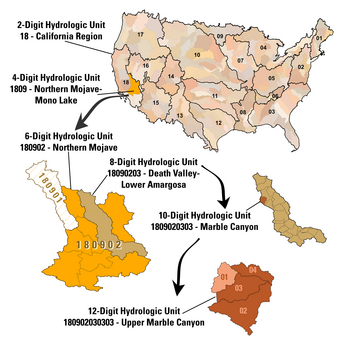
\includegraphics[width=\textwidth]{img/WBD_Base_HUStructure_small.png}
\end{column}
\end{columns}
\end{frame}

% ---------------------------------------------------------------- 15
\begin{frame}{MR violations are common; MCL violations barely exist}
\pressum{violation_binary_days_panels_k2}
\takeaway{Nitrate MR 5.7\%, arsenic 3.7\%, IOC 4.3\% of utility-years. MCL violations: 12, 5, and 32 events across 1985--2005.}
\end{frame}

% ================================================================
\section{Does coal mining contaminate utility water?}
% ================================================================

% ---------------------------------------------------------------- 17
\begin{frame}{Design: cumulative production, measured concentrations}
\begin{equation*}
\textit{Concen}_{ct}= \beta\cdot\!\!\sum_{\tau=1985}^{t}\!\!\text{UpstreamCoalProd}_{c\tau} + \rho_c + HUC02_c\cdot\tau_t + \epsilon_{ct}
\end{equation*}
\begin{itemize}\small
    \item $\textit{Concen}_{ct}$: mean annual concentration at utility $c$, year $t$ (SYR2, 1998--2005).
    \item $\beta$: effect of 10 million additional cumulative short tons mined upstream since 1985.
    \item $\rho_c$: utility fixed effects. $HUC02_c\cdot\tau_t$: watershed-region-specific year effects, absorbing region-wide industrial trends.
    \item SEs clustered at the utility level.
\end{itemize}
\medskip
\begin{itemize}
    \item Continuous treatment, \textbf{no control}: identification comes from relative exposure.
    \item Assumption: utility with large upstream production changes would have trended like those with small ones.
\end{itemize}
\end{frame}

% ---------------------------------------------------------------- 18
\begin{frame}{Mining raises contaminant levels --- but not above the limit}
\presreg{6yr_huc02fe_inorg_ravalli_2005_k2}
\takeaway{Nitrate $+$0.10 mg/L per 10M tons (***): 12.9\% of its mean. Selenium $+$0.0004 mg/L (**): 8.5\% of its mean. Arsenic and barium show no significant change. \textbf{Every reading in the sample stays under its MCL.}}
\end{frame}

% ================================================================
\section{Do utilities keep self-reporting?}
% ================================================================

% ---------------------------------------------------------------- 20
\begin{frame}{IV design: the ARP as a shifter of where coal is mined}
First stage:
\begin{equation*}
\begin{split}
\text{NumMines}_{ct} &= \alpha_0 + \alpha_1\text{NumFacility}_{ct} + \alpha_2\text{UpstreamCoalSulfur\%}_c \cdot \text{Post95}_t \\
&\quad + Y_t + C_c + \nu_{ct}
\end{split}
\end{equation*}
Second stage:
\begin{equation*}
\text{Violation}_{vct} = \beta_0 + \beta_1\text{NumFacility}_{ct} + \gamma\widehat{\text{NumMines}}_{ct} + Y_t + C_c + \epsilon_{ct}
\end{equation*}
\begin{itemize}\small
    \item $\text{Post95}_t = \mathbf{1}\{t > 1995\}$. Sulfur is time-invariant, so $C_c$ absorbs its level.
    \item Outcome: 1 if utility $c$ had a violation of type $v$ at any point in year $t$. Coefficients are in percentage points.
    \item SEs clustered at the utility level.
\end{itemize}
\end{frame}

% ---------------------------------------------------------------- 21
\begin{frame}{Shift in location of coal production w.r.t. sulfur}
\presfig[0.74\textheight]{scatterhuccoalsulfur_pooled.png}
\end{frame}

% ---------------------------------------------------------------- 22
\begin{frame}{First stage: high sulfur watersheds lost their mines}
\presreg[width=1.3\textwidth]{fs_dwnstrm_minevio_ivsum_k2}
%\takeaway{$F = 27.5$, above the 23.1 critical value of \cite{montielolea2013robust} for a 5\% test against 10\% worst-case bias, and well above the rule of thumb of 10 (\cite{staigerstock1997instrumental}).}
\end{frame}

% ---------------------------------------------------------------- 23
\begin{frame}{Instrument validity}
\begin{itemize}\small
    \item \textbf{Independence.} The ARP is national clean-\emph{air} law. Its scope, stringency, and 1995 date were set by national energy and emissions politics, not by any downstream utility's water quality or its influence over mine siting. Time-invariant sulfur exposure is absorbed by utility fixed effects.
    \item \textbf{Exclusion.} The threat is a post-1995 SDWA change hitting high- and low-sulfur utilities differently. National rule changes are absorbed by year effects. Directly testable: regress the number of intake facilities --- the observable proxy for the model's negligence type --- on the instrument. The coefficient is 0.05--0.06 (s.e.\ $\approx$0.04), with and without a balanced panel, and not statistically significant.
    \item \textbf{Monotonicity.} A defier is a high-sulfur watershed that expanded \emph{because} its coal was high sulfur. Scrubber adoption costs more likely leading to lost market share rather than gain; low-cost high-sulfur regions that expand anyway are never-takers. 
    %Monotonicity is pairwise in sulfur, so low- and high-sulfur areas may respond in opposite directions (\cite{angrist1994identification}).
\end{itemize}
\end{frame}

% ---------------------------------------------------------------- 24
\begin{frame}{Mining makes utilities stop reporting}
\presreg{2sls_dwnstrm_minevio_mr_ivsum_binvio_k2}
\takeaway{One more upstream mine raises MR violations by 3.9--4.9 pp for nitrates, 3.8--4.7 pp for arsenic, and 3.1--4.5 pp for IOC (across utility-year and utility-year-by-state-year fixed effects), against base rates of 5.7\%, 3.7\%, and 4.3\%. OLS estimates are far smaller --- consistent with negative omitted variable bias, as expected if utilities that can keep mines out are also better at compliance.}
\end{frame}

% ---------------------------------------------------------------- 25
\begin{frame}{Little record of exceedances}
\presreg{2sls_dwnstrm_minevio_mcl_ivsum_binvio_k2}
\takeaway{Nitrate and IOC MCL effects are statistically indistinguishable from zero. Arsenic rises by a small but significant $+$0.08 to $+$0.22 pp. This is not strong evidence the water stayed clean: without a self-report, the regulator cannot issue an MCL violation at all, and the arsenic result shows an exceedance can still surface. It is also the wrong prediction for concealment --- hiding is worth paying for when an exceedance is at stake, and measured concentrations are almost always below that threshold.}
\end{frame}

% ---------------------------------------------------------------- 26
\begin{frame}{Reporting cost, not concealment: Corollary 1 in the data}
\begin{itemize}\small
    \item Nitrate rules require \textbf{more frequent monitoring} once a reading exceeds 50\% of the MCL --- a discrete jump in $c$, with no jump in the penalty for under-reporting and no exceedance yet: a reading at half the limit is still a reading under the limit.
    \item Exceedance risk is held fixed (Channel B = 0), reporting cost increases (Channel A $\geq 0$).
\end{itemize}
\presreg{mr_concentration_lag_ols_k2}
\takeaway{Crossing 50\% of the nitrate MCL raises the probability of failing to report within six months by 26 pp, and within a year by 59 pp. Descriptive, not causal --- read the sign not magnitude. Utilities under-report when self-reporting gets expensive, not hiding.}
\end{frame}

% ================================================================
\section{How do regulators respond?}
% ================================================================

% ---------------------------------------------------------------- 28
\begin{frame}{Enforcement does not counteract under-reporting}
\presreg{h3_inf_formal_d12_k2}
\takeaway{One more upstream mine reduces formal enforcement by 3.4 pp with utility and year fixed effects alone (significant), but the effect loses significance once state $\times$ year fixed effects are added; informal enforcement is not significant in either specification.}
\end{frame}

% ---------------------------------------------------------------- 29
\begin{frame}{The regulator increases inspections, not enforcement}
\presreg{h2_snsv_d12_k2}
\takeaway{Only inspection visits rise significantly ($+$2.1 pp); sanitary and enforcement visits are not statistically distinguishable from zero. Regulators do not systematically step up the visit types tied to sanctions. Either there are no hidden exceedances, or visits do not find them (\cite{mi2026technology}); I cannot separate the two, but concealment is unlikely given the MCL results. Either way the penalty for under-reporting does not increase, which Proposition 3 says would work.}
\end{frame}

% ---------------------------------------------------------------- 30
\begin{frame}{Conclusion}
\begin{itemize}\small
    \item Exogenous contamination raises the cost of self-reporting, and self-reporting falls --- \textbf{even where the quality standard is never breached}.
    \item The evidence points to cost avoidance, not concealment. Corollary 1 makes the two separable: with exceedance risk held fixed, only the cost channel can move under-reporting ---  I find flat exceedance and increasing self-reporting costs.
    \item Enforcement response is mixed and fixed-effects-sensitive: formal action falls with baseline fixed effects but loses significance once state $\times$ year effects are added, and only inspection visits rise significantly --- the regulator's response does not robustly keep pace with contamination.
    \item \textbf{Policy.} Tightening MCLs does nothing if nobody tests. Self-reporting penalties are a lever to reduce under-reporting.
    %\item \textbf{Policy.} Tightening MCLs does nothing if nobody tests. By Proposition 3 the binding lever is the price of \emph{not} reporting where source water is impaired, and it is not currently being pulled (\cite{malik1993self}; \cite{harford1987self}).
    \item Open question: if regulator monitoring is more efficient than self-reporting.
\end{itemize}
\vfill
\centering \small ek559@cornell.edu
\end{frame}

% ================================================================
% Appendix
% ================================================================
\begin{frame}
\vfill
\centering
\begin{beamercolorbox}[sep=8pt,center,shadow=true,rounded=true]{title}
\usebeamerfont{title}Appendix\par
\end{beamercolorbox}
\vfill
\end{frame}

\begin{frame}{Appendix: combined MR and MCL violations}
\presreg{2sls_dwnstrm_minevio_allcat_ivsum_binvio_k2}
\takeaway{The combined effect mirrors the MR effect: nitrate 3.9--4.9 pp, arsenic 4.0--4.8 pp, IOC 3.1--4.4 pp across the two fixed-effects specifications.}
\end{frame}

\begin{frame}{Appendix: instrument balance on intake facilities}
\presreg{exclusion_test_num_facilities_k2}
\end{frame}

\begin{frame}{Appendix: concentration summary statistics}
\pressum{6yr_huc02fe_inorg_val_sumstats_ravalli_2005_k2}
\end{frame}

\begin{frame}{Appendix: who appears in the Six-Year Review}
\pressum{syr2_mr_comparison_k2}
\takeaway{Utilities with SYR2 readings are 7--14 pp more likely to ever incur an MR violation. The concentration sample over-represents the more negligent utilities, so it is not selected toward clean systems.}
\end{frame}

\begin{frame}{Appendix: enforcement and visits in the panel}
\pressum{enforcement_visit_type_panels_k2}
\takeaway{Enforcement responds to violations --- any enforcement rises from 21\% overall to 71\% in MR years --- but sanitary visits are no more likely in MR years than in any other year.}
\end{frame}

\begin{frame}{Appendix: where coal production moved, 1985--2005}
\presfig[0.72\textheight]{proportionatecircleprod_diff_allminehuc12_1985_2005.png}
\end{frame}

\begin{frame}{Appendix: residualized first stage}
\presfig[0.72\textheight]{first_stage_scatter_dwnstrm.png}
\end{frame}

\begin{frame}{Appendix: sample watersheds}
\presfig[0.72\textheight]{map_huc12_main_sample.png}
\end{frame}

\begin{frame}{Appendix: Corollary 1, statement and proof}
\footnotesize
Write the share of types under-reporting as $h(\theta,m) = 1 - G(c^*(\theta);m)$, with cutoff $c^*(\theta) = t - (r-ps)\,q(a_{SR}(\theta))$, so that
\[
\frac{\partial MR}{\partial m} = \underbrace{\int_0^{\bar\theta}\!\frac{\partial h(\theta,m)}{\partial m}\,f(\theta;m)\,d\theta}_{\text{A: cost}} \;+\; \underbrace{\int_0^{\bar\theta}\! h(\theta,m)\,\frac{\partial f(\theta;m)}{\partial m}\,d\theta}_{\text{B: composition}}.
\]
\textbf{Corollary 1.} If $q(a_{SR}(\theta)) \equiv \bar q$ on $(0,\bar\theta)$, then $\partial MR/\partial m = -\,\partial G(\bar c;m)/\partial m \ge 0$, where $\bar c = t-(r-ps)\bar q$.
\smallskip

\textit{Proof.} The cutoff is then type-invariant, $c^*(\theta) \equiv \bar c$, so $h(\theta,m) = 1-G(\bar c;m)$ does not vary with $\theta$ and comes outside both integrals. The limits $0$ and $\bar\theta$ do not depend on $m$, so by Leibniz's rule
\[
\text{B} = \big[1-G(\bar c;m)\big]\,\frac{d}{dm}\!\left[\int_0^{\bar\theta}\! f(\theta;m)\,d\theta\right] = \big[1-G(\bar c;m)\big]\,\frac{d}{dm}[1] = 0,
\]
since $f(\cdot\,;m)$ is a density for every $m$. Channel A collapses to $-\,\partial G(\bar c;m)/\partial m \ge 0$, because contamination shifts reporting costs up. $\square$
\smallskip

\textbf{Why it matters.} Channel B is the concealment margin: it operates only if contamination reallocates mass toward types whose exceedance risk, and hence whose cutoff, differs. Shut it down and any remaining rise in under-reporting is avoidance of the reporting technology itself. The 50\%-of-MCL nitrate step is the empirical counterpart --- monitoring frequency jumps, the sanction schedule does not, and readings are nowhere near the limit.
\end{frame}

\begin{frame}[allowframebreaks]{References}
\printbibliography
\end{frame}

\end{document}
